% !TEX TS-program = pdflatex
% !TEX encoding = UTF-8 Unicode

% This is a simple template for a LaTeX document using the "article" class.
% See "book", "report", "letter" for other types of document.

\documentclass[11pt]{article} % use larger type; default would be 10pt

\usepackage[utf8]{inputenc} % set input encoding (not needed with XeLaTeX)

%%% Examples of Article customizations
% These packages are optional, depending whether you want the features they provide.
% See the LaTeX Companion or other references for full information.

%%% PAGE DIMENSIONS
\usepackage{geometry} % to change the page dimensions
\geometry{a4paper} % or letterpaper (US) or a5paper or....
% \geometry{margin=2in} % for example, change the margins to 2 inches all round
% \geometry{landscape} % set up the page for landscape
%   read geometry.pdf for detailed page layout information

\usepackage{graphicx} % support the \includegraphics command and options

% \usepackage[parfill]{parskip} % Activate to begin paragraphs with an empty line rather than an indent

%%% PACKAGES
\usepackage{tikz}
\usepackage{booktabs} % for much better looking tables
\usepackage{color} % Added by me
\usepackage{array} % for better arrays (eg matrices) in maths
\usepackage{paralist} % very flexible & customisable lists (eg. enumerate/itemize, etc.)
\usepackage{verbatim} % adds environment for commenting out blocks of text & for better verbatim
\usepackage{subfig} % make it possible to include more than one captioned figure/table in a single float
% These packages are all incorporated in the memoir class to one degree or another...

%%% HEADERS & FOOTERS
\usepackage{fancyhdr} % This should be set AFTER setting up the page geometry
\pagestyle{fancy} % options: empty , plain , fancy
\renewcommand{\headrulewidth}{0pt} % customise the layout...
\lhead{}\chead{}\rhead{}
\lfoot{}\cfoot{\thepage}\rfoot{}

%%% SECTION TITLE APPEARANCE
\usepackage{sectsty}
\allsectionsfont{\sffamily\mdseries\upshape} % (See the fntguide.pdf for font help)
% (This matches ConTeXt defaults)

%%% ToC (table of contents) APPEARANCE
\usepackage[nottoc,notlof,notlot]{tocbibind} % Put the bibliography in the ToC
\usepackage[titles,subfigure]{tocloft} % Alter the style of the Table of Contents
\renewcommand{\cftsecfont}{\rmfamily\mdseries\upshape}
\renewcommand{\cftsecpagefont}{\rmfamily\mdseries\upshape} % No bold!

%%% END Article customizations

%%% The "real" document content comes below... %%%

\title{Tournaments and Cycles}
\author{Ethan Schaffer}
\date{Due 10/13/16}
\newcommand\tab[1][1cm]{\hspace*{#1}}

\begin{document}
\maketitle

\section{Problem}
Prove that a tournament is intransitive if and only if it contains a directed cycle.

To solve this problem, I used what I learned from 4.8.2, 4.8.3, and 4.8.4. 

\section*{Problem 4.8.2}
\textit{How many tournaments are there with n teams?}
\\ \tab There are $2^{\frac{(n)(n-1)}{2}}$ tournaments that are possible for a tournament of n teams. 
This is because for every extra edge (represented by $\frac{(n)(n-1)}{2}$), there are 2 times the possibilties.

\section*{Problem 4.8.3}
\textit{Is the tournament in Figure 4.33 transitive or intransitive?}
The tournament in 4.33 is intransitive. A, D, and E all lose to one of their opponents, but beat the other.

\section*{Problem 4.8.4}
\textit{Give an example of a transitive tournament with five teams.}\\
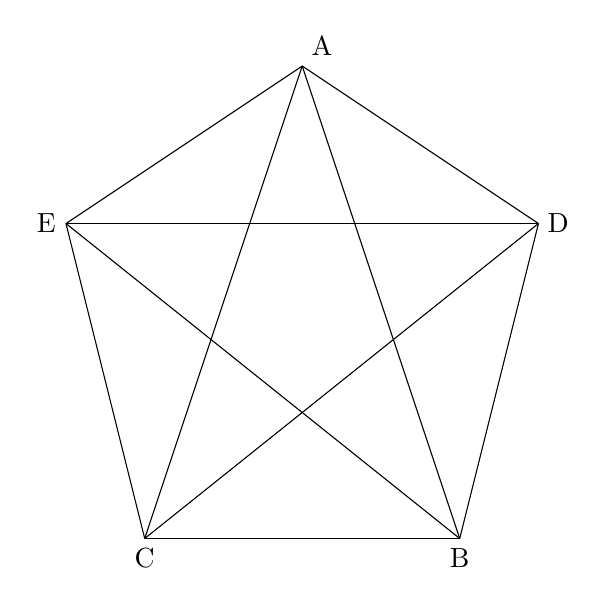
\begin{tikzpicture}
\draw(0.25,3.25) node {A};
\draw(2,-3.25) node {B};
\draw(-2,-3.25) node {C};
\draw(3.25,1) node {D};
\draw(-3.25,1) node {E};
\draw (0, 3) -- (2, -3);
\draw (0, 3) -- (-2, -3);
\draw (0, 3) -- (3, 1);
\draw (0, 3) -- (-3, 1);
\draw(2, -3) -- (3,1);
\draw(2, -3) -- (-3,1);
\draw(-2, -3) -- (3,1);
\draw(-2, -3) -- (-3,1);
\draw(-2, -3) -- (2, -3);
\draw(-3, 1) -- (3,1);
\end{tikzpicture}

\section*{Prove that a tournament is intransitive if and only if it contains a directed cycle.}
We know that any tournament with a directed cycle will have a 'loop' of points, which is how I will begin this proof.
\\
\begin{tikzpicture}
\draw(1.25,1.25) node {A};
\draw(1.25,-1.25) node {B};
\draw(-1.25,1.25) node {C};
\draw(-1.25,-1.25) node {D};
\draw (1, 1) -- (1 ,-1);
\draw (1, 1) -- (-1, 1);
\draw (-1,-1) -- (1, -1);
\draw (-1,-1) -- (-1, 1);
\draw [->] (1, 1) -- (0,1);
\draw [->] (-1, 1) -- (-1, 0);
\draw [->] (-1,-1) -- (0, -1);
\draw [->] (1,-1) -- (1, 0);
\draw (0, -2) node {Fig. 1};
\end{tikzpicture} \\
In figure 1, we have begun to draw a tournament. However, we have to make it into a complete graph for us to count it as a tournament.

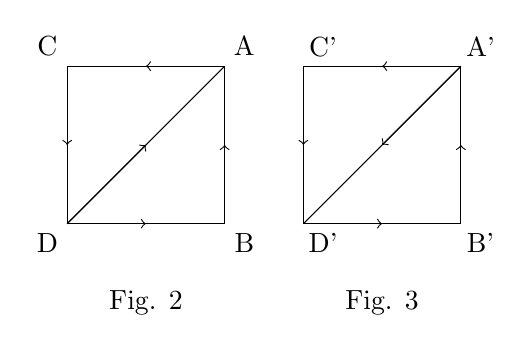
\begin{tikzpicture}
\draw(1.25,1.25) node {A};
\draw(1.25,-1.25) node {B};
\draw(-1.25,1.25) node {C};
\draw(-1.25,-1.25) node {D};
\draw (1, 1) -- (1 ,-1);
\draw (1, 1) -- (-1, 1);
\draw (-1,-1) -- (1, -1);
\draw (-1,-1) -- (-1, 1);
\draw [->] (1, 1) -- (0,1);
\draw [->] (-1, 1) -- (-1, 0);
\draw [->] (-1,-1) -- (0, -1);
\draw [->] (1,-1) -- (1, 0);
\draw [->] (-1,-1) -- (0,0);
\draw (-1,-1) -- (1,1);

\draw (0, -2) node {Fig. 2};

\draw(4.25,1.25) node {A'};
\draw(4.25,-1.25) node {B'};
\draw(2.25,1.25) node {C'};
\draw(2.25,-1.25) node {D'};
\draw (4, 1) -- (4 ,-1);
\draw (4, 1) -- (2, 1);
\draw (2,-1) -- (4, -1);
\draw (2,-1) -- (2, 1);
\draw [->] (4, 1) -- (3,1);
\draw [->] (2, 1) -- (2, 0);
\draw [->] (4,-1) -- (4, 0);
\draw [->] (2,-1) -- (3, -1);
\draw (4, 1) -- (2,-1);
\draw [->] (4, 1) -- (3,0);

\draw (3, -2) node {Fig. 3};
\end{tikzpicture}
\\
Here, we have drawn $\overline{AD}$ and $\overline{A'D'}$. No matter which team we have win, we create a directed 3 cycle. This concept works for larger shapes as well. For a directed \textit{n} cycle, we can always connect two points which are adjacent to the same point. If we connect it with one result, we have created a directed 3 cycle. If we have to opposite team win, we have created a directed \textit{n-1} cycle, which we can then apply to same technique on. 

\section{Analysis}
This problem was very interesting, and tournaments have been a cool way to apply graph theory. I hope we will talk about brackets soon - they seem very interesting. 
\section{Status}
I feel like I understand this problem very well, and am excited to prove more cool things about tournaments. 
\section{MVP}
I have no MVP.
\end{document}
